\documentclass{article}

\usepackage{amssymb}
\usepackage{amsfonts}
\usepackage[tbtags]{amsmath}
\usepackage{amscd}
\usepackage{amsthm}			% Продвинутая математика
\usepackage{mathtext}
\usepackage{cmap}
\usepackage[T2A]{fontenc}
\usepackage[utf8]{inputenc}			% cp1251
\usepackage[english, russian]{babel}
%\usepackage{literat}
\usepackage{pifont}
\usepackage{bm}
\usepackage{array}			% Ширина столбиков в массиве
\usepackage{dcolumn}
\usepackage{hhline}
\usepackage{multirow}
\usepackage{graphicx}
\usepackage{rotating}
\usepackage{calc}
\usepackage{tabularx}
\usepackage{afterpage}
\usepackage{ifthen}
\usepackage{caption2}
\usepackage{substr}
\usepackage[mathscr]{eucal}  %% My addition
\usepackage{mathrsfs}        %% My addition
\usepackage{hypbmsec}        %% My addition
\usepackage{latexsym}        %% My addition
\usepackage{xypic}           %% My addition
\RequirePackage{soul}
\RequirePackage{verbatim}    %% My addition
\RequirePackage{chapterbib}
\RequirePackage{enumerate}

\usepackage[shortcuts]{extdash}
\usepackage{ragged2e}
\usepackage{etoolbox}
\usepackage{lipsum}

%\usepackage{flafter}
\usepackage[section,above,below]{placeins}

\usepackage{indentfirst}
\usepackage[a4paper, top=20mm, left=30mm, right=20mm, bottom=25mm]{geometry}

\title{Исследование влияния весовых коэффициентов при решении задачи идентификации проницаемости для нефтяного месторождения}
\author{V.P. Kosyakov}


\begin{document}
	\maketitle
	\textbf{Abstract}. В процессе моделирования разработки нефтяного месторождения одним из важных шагов является решение обратной задачи, решение которой, как правило, заключается в подборе параметров модели для наилучшей настройки на историю разработки. Для решения обратной задачи используются разнородные исходные данные, степень влияния на результат решения которых определяется их весовыми коэффициентами. Кроме того целью моделирования является не только повторение показателей разработки на историческом периоде, но и получение достоверного прогноза поведения моделируемого объекта в будущем. 
	В настоящей  работе на примере решения задачи параметрической идентификации поля проницаемости для моделирования разработки нефтяного месторождения проведено исследование влияния выбора весовых коэффициентов на точность настройки модели и её прогнозные характеристики. Показано, что корректный выбор весовых коэффициентов позволяет получить модель с наилучшими прогнозными свойствами. Для оценки точности модели и выбора варианта её адаптации рекомендовано использовать дополнительные метрики отличные от целевой функции.

\textbf{Keywords}: обратная задача, параметрическая идентификация, моделирование, фильтрация, метрика

\section{INTRODUCTION}
	В настоящее время широкое распространение получило создание цифровых (численных) двойников всевозможных объектов и физических процессов, в основе которых, как правило, лежат математические модели. Для успешного использования подобных моделей на практике необходимым условием является воспроизведение фактического поведения исследуемого объекта. Для удовлетворения этого требования численные модели проходят процедуру настройки (адаптации), которая представляет собой решение обратной задачи с целью подбора некоторых параметров модели, а также начальных и/или граничных условий, если они не известны с достаточной точностью. 
	
	Применительно к задачам фильтрации, подземной гидродинамики, разработки нефтяных месторождений актуальной задачей является задача восстановления поля проницаемости. Ввиду малого объёма знаний о истинном поле проницаемости породы, данные о котором непосредственно могут быть получены лишь при бурении скважин, значение проницаемости в межскважинном пространстве является оценочным. Значение проницаемости является одним из  важных параметров, характеризующих потенциал и процесс разработки месторождения. Следовательно, задача восстановления или уточнения поля проницаемости является актуальной задачей. При использовании гидродинамической модели и известных фактических значениях основных показателей разработки на историческом периоде (отборы жидкости, нефти, закачка воды, пластовые и забойные давления и т.д.), становится возможным получение решения обратной задачи. Решение заключается в нахождении такого поля проницаемости, при использовании которого расчётные значения показателей удовлетворяют с достаточной точностью фактическим данным.

	В настоящей работе представлено исследование зависимости адаптационных и прогнозных характеристик модели от степени доверия к исходным данным разного вида. В работах \cite{mus}, \cite{kos} продемонстрирована не прямая зависимость точности прогноза от точности настройки модели на историю. На примере задачи параметрической идентификации фильтрационной модели для нефтяного месторождения в двухфазной постановке, показана важность использования всего объёма исходных данных. В качестве прогнозируемого параметры выступает пластовое давление, характеризующее “энергетический” потенциал залежи и расходы воды.

\section{Mathematical Models}
Для решения поставленной задачи в качестве фильтрационной модели использовалась двумерная математическая модель фильтрации несжимаемой "цветной" жидкости \cite{bas}. Использование модели цветной жидкости предполагает: одинаковую вязкость жидкостей равную $\mu$, прямо пропорциональную зависимость относительной фазовой проницаемости от насыщенности соответствующей фазой, отсутствие влияния насыщенности на давление, капиллярные силы не учитываются, давление фаз принимается равным. Таким образом уравнения фильтрации можно записать следующим образом: 
\begin{equation} \label{fil}
\triangledown\frac{k}{\mu}\triangledown P = \delta_{l}(x,y),
\end{equation}
\begin{equation} \label{fil2}
\frac{\phi\partial S_w}{\partial t} = \triangledown\frac{kk_{rw}}{\mu}\triangledown P +\delta_w(x,y),
\end{equation}
\begin{equation} \label{bc}
\delta_{i}(x,y)  = \left\{\begin{array}{crl}
0, \;при\;(x,y) \notin\ \Gamma_{in}\cup\Gamma_{out}\\
q_{i\:k}, \;при\;(x,y) \in \Gamma_{in}\\
q_{i\:aq}, \;при\;(x,y) \in \Gamma_{out}
\end{array}\right.,
\end{equation}
\begin{equation*}
	i = l,w.
\end{equation*}
Замыкающие соотношения:
\begin{equation*}
	S_w + S_o = 1,
\end{equation*}
\begin{equation} \label{kr}
	k_w = S_w, \quad k_o = 1 - S_w,
\end{equation}
\begin{equation*}
	P = P_0,\quad S_w = S_{w0}\mbox{,\quad при $t=0$},
\end{equation*}
где $k$ - проницаемость, $P$ - пластовое давление, $\phi$ - пористость, $S$ - насыщенность, нижний индекс $i$ обозначает $l$ - жидкость (вода и нефть), $w$ - вода, или  $k_{r}$ - относительная фазовая проницаемость, $q_k$ - расход флюида в $k$-той скважине, $\Gamma_{in}$ - множество координат источников/стоков (скважин), $\Gamma_{out}$ - внешняя граница, $P_0$ - пластовое давление и $S_{w0}$ - водонасыщенность в начальный момент времени $t=0$, $q_{aq}$ - удельный расход флюида через внешнюю границу, который находится по формуле:

\begin{equation*} \label{qaq}
q_{i\:aq} = \lambda \frac{kk_{ri}}{\mu}(P|_{\Gamma_{out}}-P_c),
\end{equation*}
где $P_{c}$ - на контуре питания ($P_c = P_0$), $\lambda$ - коэффициент продуктивности аквифера. Предполагается, что водонасыщенность контура питания $S_{c\:w} = 1$.
Решение обратной задачи заключается в поиске поля проницаемости $k = k(x,y)$ при котором расчётные значения пластового давления и расхода воды на скважинах будут удовлетворительно совпадать с исходными значениями соответствующих параметров. Обратная задача решается в оптимизационной постановке, которая заключается в минимизации целевой функции $J$. Целевую функцию можно записать в виде суммы слагаемых, каждое из которых является произведением функции характеризующей отклонение расчётных значений от контрольных и весового коэффициента для соответствующего типа переменной. В качестве меры отклонения выбрана средняя квадратичная ошибка "Mean Squared Error" (MSE). 
\begin{equation} \label{mse}
	J=w_p\frac{1}{N}\sum_{i=1}^N{\left(p_c^i-p_f^i\right)^2}+w_{q_w}\frac{1}{M}\sum_{i=1}^M{\left(q_{w\:c}^i-q_{w\:f}^i\right)^2}
\end{equation}
где $p_c^i$ -расчетное значение пластового давления, $p_f^i$ - фактическое значение, $i$ - номер замера, $N$ - количество замеров пластового давления, $q_{w\:c}^i$ и $q_{w\:f}^i$ - расчетное и фактическое значение расхода воды на скважинах соответственно, нижний индекс $f$ означает фактические значения (fact), а $c$ - расчётные (calculated), $M$ - количество замеров расхода воды на скважине, $w_p$ и $w_{q_w}$- весовые коэффициенты учитывающие степень влияния различных параметров (размерность, качество данных и т.д.). Аргументами слагаемого целевой функции отвечающего за давление выступают фактические (замеренные) и расчётные значения пластового давления в точках расположения скважин в заданные моменты времени.  
 Расчётные значения в свою очередь зависят от параметров модели $u$. Решение находится при использовании градиентного оптимизационного алгоритма и заключается в определении набора параметров модели соответствующих минимуму $J$ и удовлетворяющих ограничениям в виде неравенств:
\begin{equation*}
u_{min}\leq\ \boldsymbol{u}\leq u_{max},
\end{equation*}
$u_{min}$ и $u_{max}$ - минимальный и максимальные значения для каждого параметра.

При использовании градиентного метода оптимизации, необходимо найти компоненты градиента целевой функции, которые можно записать в следующем виде:
\begin{equation}\label{grad}
\frac{\partial J}{\partial u_k} = 2w_p\frac{1}{N}\sum_{i=1}^N ({p_c^i-p_f^i})\frac{\partial p_c^i}{\partial u_k}+2w_{q_w}\frac{1}{M}\sum_{i=1}^M{\left(q_{w\:c}^i-q_{w\:f}^i\right)}\frac{\partial q_{w\:c}^i}{\partial u_k}.
\end{equation}
Для решения оптимизационной задачи необходимо чтобы каждая компонента градиента целевой функции стремилась к 0, что можно записать как:
\begin{equation} \label{rp}
	 \frac{\partial J}{\partial u_k} \rightarrow 0
\end{equation}
Решение обратной задачи (\ref{rp}) находится численно итерационным методом. На каждой итерации численно решается прямая задача (\ref{fil}-\ref{bc}) и осуществляется расчёт производных целевой функции по настраиваемым параметрам модели \cite{opt}. Численное решение находилось методом контрольного объёма  для двумерной прямоугольной разностной сетки при использовании IMPES метода \cite{azi}.

Для расчёта слагаемого компоненты градиента целевой функции (\ref{grad}), отвечающего за отклонение расходов фаз (воды) необходимо его преобразовать к виду, где множитель $\frac{\partial q_{w\:c}^i}{\partial u_k}$ будет выражен через производную пластового давления от параметра $u_k$. Для модели цветных жидкостей расход воды можно выразить через расход жидкости и относительную фазовую проницаемость как:
 \begin{equation*}
 	q_{w\:c}^i = k_{w}^i \: q_{w\:c}^i.
 \end{equation*}
С учётом (\ref{bc}, \ref{kr}) производная относительной фазовой проницаемости воды по водонасыщенности:
 \begin{equation*}
	\frac{\partial k_{w}^i}{\partial s_w^i} = 1,
\end{equation*}
где $s_w^i$ - водонасыщенность в прискважинной области.
Тогда множитель $\frac{\partial q_{w\:c}^i}{\partial u_k}$ записывается как:
\begin{equation} \label{dq_du}
\frac{\partial q_{w\:c}^i}{\partial u_k} = k_{w}^i \frac{\partial q_{l\:c}^i}{\partial u_k} + q_{l\:c}^i \frac{\partial k_{w}^i}{\partial u_k} = q_{l\:c}^i \frac{\partial k_{w}^i}{\partial s_w^i} \frac{\partial s_w^i}{\partial p_c^i}\frac{\partial p_c^i}{\partial u_k} =  q_{l\:c}^i  \frac{\partial s_w^i}{\partial p_c^i}\frac{\partial p_c^i}{\partial u_k}.
\end{equation}
В используемой модели на скважинах задаются расходы жидкости, то первое слагаемое в (\ref{dq_du}) равняется 0, так как настраиваемый параметр (управление) $u_k$ не может влиять на значение расходов жидкости. В случает решения задачи при заданных забойных давлениях это слагаемое необходимо учитывать.

Основная вычислительная сложность заключается в вычислении значений $\frac{\partial p_c^i}{\partial u_k}$ и $\frac{\partial s_w^i}{\partial p_с^i}$. Их расчёт выполняется численно при использовании уравнений (\ref{fil} - \ref{fil2}) и на основе подхода \cite{opt}. Используемый алгоритм расчёта производных возможен для применения с другими техниками восстановления поля проницаемости \cite{leg}.

Целевая функция, используемая при решении обратной задачи ({\ref{mse}}), не всегда удобна при субъективной оценке точности модели. Оценка точности настройки модели, в качестве дополнительной метрики, производилась при помощи показателя - средняя абсолютная ошибка в процентах "Mean Absolute Percentage Error" (MAPE). Для показателей "пластовое давление" и  "расход воды" эти метрики можно представить следующим образом:

\begin{equation*} \label{mape_p}
 	J_{mape(p)}=\frac{1}{N}\sum_{i=1}^N{\left|\frac{p_c^i-p_f^i}{p_f^i}\right|},
\end{equation*}
\begin{equation*} \label{mape_qo}
 	J_{mape(q_w)}=\frac{1}{M}\sum_{i=1}^M{\left|\frac{q_{w\:c}^i-q_{w\:f}^i}{q_{w\:f}^i}\right|}.
\end{equation*}
Данная метрика позволяет наглядно дать оценку качеству воспроизведения моделью фактических значений пластового давления и расхода воды на скважинах.
\section{Сalculation Results}
На примере решения обратной задачи поиска поля проницаемости для нефтяного месторождения было выполнено исследование зависимости качества адаптации и прогноза от соотношения весовых коэффициентов отражающих влияние исходных данных. Для выполнения исследования при помощи синтетической гидродинамической модели был получен необходимый набор данных (показателей разработки): пластовые давления и расходы воды на скважинах. Для синтетической модели были заданы размеры расчётной области, расположение скважин начальные и граничные условия, в том числе режимы работы скважин (расходы жидкости на скважинах), а также исходное поле проницаемости. Полученные расчётные данные выступали в качестве "фактических" значений, которые использовались при решении обратной задачи. Схема расположения скважин представлена на рисунке \ref{fig:map}, размеры указанны в метрах. 
\begin{figure}
	\center{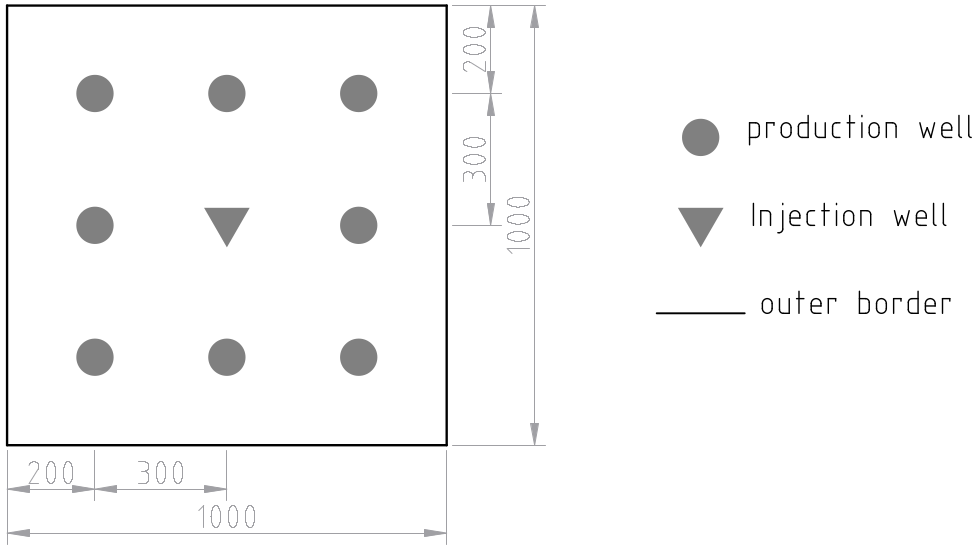
\includegraphics[height=12pc]{fig1.png}}
    \caption{Схематическое представление расчётной области.}
	\label{fig:map}
\end{figure}

Месторождение разрабатывается при помощи 8 добывающих и 1 нагнетательной скважины. На скважинах задавался расход жидкости (дебит на добывающих и приёмистость на нагнетательных), Расход жидкости на каждой скважине задавался в виде зашумлённого фиксированного значения, амплитуда шума составляла до $50\%$ от среднего значения. Шаг по времени составлял 1 месяц. Период разработки - 30 лет, контур питания был “подключён” по периметру расчетной области. Для решения задачи параметрической идентификации период разработки был разбит на 2 интервала: интервал адаптации, на котором настраивались параметры модели, и интервал валидации, на котором оценивались прогнозные характеристики адаптированной модели. Периоды составляли 20, 10 лет соответственно. Объём исходных данных, который использовался при настройке модели на интервале адаптации составляет 63 значений давления случайно выбранных из всего объёма исходных значений давлений на скважинах, что составляет примерно $2,5\%$ от доступного числа. Для интервала адаптации использовалось 1920 значения расхода воды на добывающих скважинах. На интервале валидации объём исходных данных составлял 37 и 960 значения для давления и расхода соответственно. 

Прямая и обратная задача решались численно методом контрольного объёма, разностная сетка имела 441 расчётный узел, каждый узел имеет своё значение проницаемости, которое является настраиваемым параметром.

Задача адаптации решается для 11 вариантов наборов весовых коэффициентов $(w_p, w_{q_w})$ используемых в целевой функции {\ref{mse}}. Значения весовых коэффициентов в наборах задавалось таким образом чтобы выполнялось условие $w_p = 1 - w_{q_w}$, где $w_{q_w}$ изменялось от 0 до 1 с шагом 0,1. Путём изменения весовых коэффициентов менялась чувствительность целевой функции и её градиента к разным видам исходных данных. Кроме того, при значении одного из весовых коэффициентов равным 0, модель настраивается только на один из двух видов исходных данных. 

Методология проведения исследования: задаётся поле проницаемости, задаются режимы работы скважин (расходы жидкостей), решается прямая задача, расчётные значения пластового давления и расхода нефти сохраняются и далее выступают в качестве фактических значений. Далее вносится возмущение в исходное поле проницаемости, которое выступает в качестве начального приближения при решении обратной задачи. Далее решается обратная задача с целью восстановить такое поле проницаемости что-бы максимально точно воспроизвести фактические значения пластового давления и расхода воды на скважинах с учётом заданных весовых коэффициентов. Далее адаптированная модель выполняет прогнозные расчёты, период прогноза совпадает с интервалом валидации, на котором оценивается способность модели воспроизвести интересующие нас показатели, исходные значения которых не участвовали в процессе адаптации. 

На рисунке \ref{fig:press} представлены исходные значения пластового давления для скважин в разные моменты времени, вертикальная пунктирная линия на этом графике и на последующих разделяет интервалы адаптации и валидации. На рисунке \ref{fig:qlic} представлена динамика суммарного расхода жидкости и воды для добывающих скважин, пиктограммами показаны исходные значения, линиями - осреднения динамика соответствующих показателей.
\begin{figure} 
    \begin{minipage}[h]{0.48\linewidth}
      \center{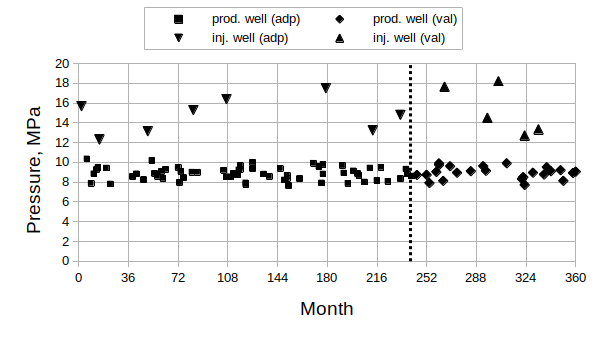
\includegraphics[height=0.60\linewidth]{fig2.png}}
      \caption{Значения пластового давления вблизи скважин для интервалов адаптации и валидации.}
      \label{fig:press}
    \end{minipage} \hfill
    \begin{minipage}[h]{0.48\linewidth}
      \center{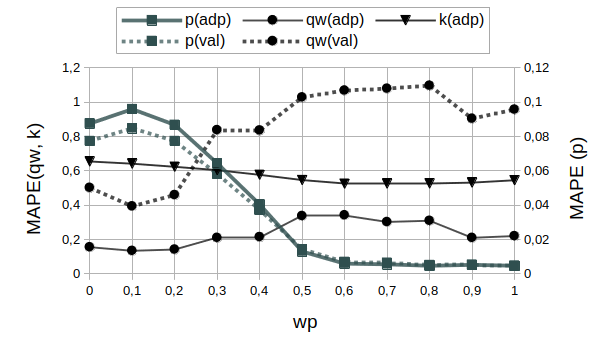
\includegraphics[height=0.60\linewidth]{fig3.png}}
      \caption{Значения суммарных расходов жидкости и воды для этапов адаптации и валидации.}
      \label{fig:qlic}
    \end{minipage} 
\end{figure}
Из рисунков видно, что средние значения пластового давления и расхода жидкости постоянны на протяжении всего периода моделирования, расход воды постепенно возрастает по мере вытеснения нефти водой и прихода фронта скачка  водонасыщенности к добывающим скважинам.

Обратная задача была решена для 11 вариантов наборов весовых коэффициентов, в которых постепенно увеличивалось влияние данных давления и уменьшалось влияние расхода воды. На рисунке \ref{fig:wp} представлены значения метрик MAPE и целевой функции $J$ для разных наборов весовых коэффициентов. Метрика MAPE рассчитана для показателей давления, расхода воды на добывающих скважинах для интервалов адаптации и валидации. Кроме того на рисунке представлена метрика MAPE для проницаемости, характеризующая отклонение восстановленных значений от фактических.

\begin{figure}
	\center{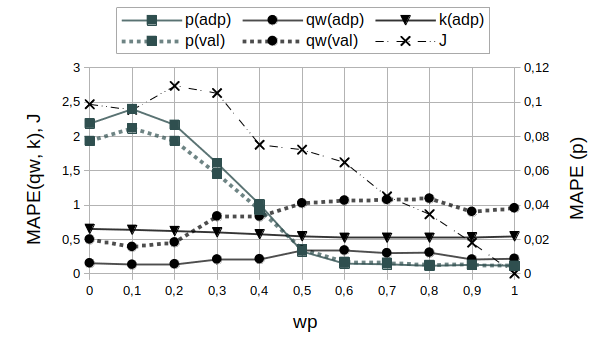
\includegraphics[height=12pc]{fig4.png}}
	\caption{Значения метрики MAPE и целевой функции J для 11 наборов весовых коэффициентов для интервалов адаптации (adp) и валидации (val)}
	\label{fig:wp}
\end{figure}

Из графика видно, что в целом наблюдается ожидаемая обратно пропорциональная зависимость значения метрики и соответствующего весового коэффициента. Также наблюдается похожее поведение соответствующих метрик для интервалов адаптации и валидации. Однако, чувствительность метрики, характеризующей прогнозные свойства для показателя "расхода воды", выше чем метрика этого же показателя на интервале адаптации, что свидетельствует о важности выбора того или иного варианта адаптации с точки зрения прогнозных свойств. Из рисунка \ref{fig:wp} также видно, что характер изменения целевой функции $J$ отличается от характера изменения метрики MAPE. Исходя из графика можно сделать вывод о том, что при изменении весового коэффициента $w_p$ в интервале от 0 до 0,3 модели наиболее тяжело удовлетворить исходным данным. Так как основной целью моделирования является получение достоверного прогноза, а так же с учётом характера зависимости метрик и их абсолютных значений от весовых коэффициентов рекомендуется выбрать вариант адаптации модели при значении весового коэффициента $w_p$ = 0.1. Также следует ответить, что ввиду особенности решения обратной задачи ни одно из решений не воспроизвело исходное поле проницаемости, отклонение составляло более 50\%, тем не менее прогнозные характеристики этих моделей являются удовлетворительными, как для пластового давления, так и для расхода воды. На практике мы не знаем настоящее поле проницаемости, и полученное для практических задач решение является приемлемым если обладает удовлетворительной настройкой на историю и хорошими прогнозными свойствами. 

Для выбранного варианта адаптации и для предельных вариантов ($w_p = 0$ и $w_p = 1$) сравним поведение дополнительного интегрального показателя - средней обводнённости на интервалах адаптации и валидации. Средняя обводнённость в каждый момент времени рассчитывается как $wtc = \frac{\sum{q_w^i}}{\sum{q_l^i}}$. Средняя обводнённость добываемой жидкости представлена на рисунке \ref{fig:wtс}. Пиктограммами на рисунке \ref{fig:wtс} нанесены значения обводнённости на каждый месяц, линиями усреднённые значения для четырёх вариантов: исходный вариант и 3 варианта адаптированной модели с весовым коэффициентом $w_p$ равными 0, 0.1 и 1. 
\begin{figure}
	\center{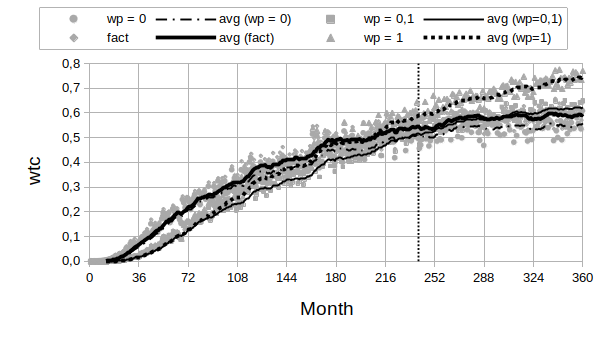
\includegraphics[height=12pc]{fig5.png}}
	\caption{Динамика обводнённости добываемой жидкости: фактические значения и для 3х вариантов адаптации модели.}
	\label{fig:wtс}
\end{figure}
Из рисунка видно, что вариант адаптации при учёте только пластового давления $(w_p=1)$ заметно отличается исходного варианта как на этапе адаптации, так и на интервале валидации. Вариант адаптации, учитывающий только расходы воды $(w_p=0)$, в меньшей степени отличается от исходного варианта, это объясняется тем, что расход фаз на скважинах зависит как непосредственно от пластового давления, так и от структуры фильтрационных потоков в межскважинном пространстве, которая в свою очередь зависит от пластового давления. Это также видно из уравнения \ref{dq_du}, где производная расхода воды от проницаемости зависит от производной давления от проницаемости. С точки зрения прогнозирования наилучшим является вариант адаптации, который комплексно учитывает давление и расход воды, пониженный весовой коэффициент $(w_p=1)$ объясняется тем, что зависимость от пластового давления, как было сказано ранее, входит в слагаемое целевой функции отвечающее за расход воды и косвенно учитывается. Тем не менее наличие слагаемого отвечающее за пластовое давление имеет значение при безводном периоде работы, когда фронт скачка водонасыщенности ещё не дошёл до добывающих скважин. Таким образом использование в качестве целевой функции суммы позволяет более полно использовать всю имеющуюся информацию на протяжении всего периода моделирования. 

\section{CONCLUSIONS}

В результате исследования было показано, что точность решения обратной задачи зависит от выбора весовых коэффициентов, характеризующих степень влияния на настройку определённого вида данных. Использование комбинации исходных данных позволяет повысить степень регуляризации задачи. Точность модели для периодов адаптации и валидации зависит от пропорций выбранных весовых коэффициентов. Зависимость точности настройки и прогнозирования для отдельного показатель не является линейной от соответствующего ему весового коэффициента. Зависимость характеризуется наличием минимумов и максимумов, что свидетельствует о том, что степень учёта разных показателей влияют на процесс настройки и могут способствовать нахождению наиболее точного решения. Ввиду особенностей методики решения обратных задач в оптимизационной постановке, которая заключается минимизации одной функции включающей в себя разнородные данные целесообразным является анализ других метрик, позволяющих оценить точность настройки и прогнозирования с другой стороны. При условии наличия набора адаптированных моделей сторонние метрики позволят выбрать наиболее подходящую модель с точки зрения предъявляемый к ней требований.


\section{FUNDING}
The research was carried out within the state assignment of Ministry of Science and Higher Education of the Russian Federation (project No. 121030500156-6).

%
% The Bibliography
%
\begin{thebibliography}{99}
\bibitem{mus} E.N.Musakaev, S.P.Rodionov, D.Y.Legostaev, V.P.Kosyakov,  «Parameter identification for sector filtration model of an oil reservoir with complex structure» // AIP Conference Proceedings 2125,030113 2019;

\bibitem{kos} V. P. Kosyakov. "Structural and Parametric Identification of an Aquifer Model for an Oil Reservoir". Lobachevskii J Math. 2020. V. 41, P. 1242–1247.

\bibitem{bas} K. S. Basniev, N. M. Dmitriev, R. D. Kanevskaya, V. M. Maksimov. \textit{Underground hydromechanics}. M.-Izhevsk: Institute for Computer Research, 2006. [in Russian]

\bibitem{azi} H. Aziz, E. Settari. \textit{Mathematical modeling of reservoir systems}.  M.-Izhevsk: Institute for Computer Research, 2004. [in Russian]

\bibitem{opt} V.P.Kosyakov, S.P.Rodionov "Optimal control of wells on the basis of two-phase filtration equations". Proceedings of MIPT. 2016. V. 8, N 3. P. 79–90.

\bibitem{leg} V. P. Kosyakov,  D. Yu. Legostaev.“Using elements of machine learning to
solve the inverse problem of reconstructing the hydraulic conductivity feld for a fltration
problem”. Tyumen State University Herald. Physical and Mathematical Modeling. Oil, Gas,
Energy, V. 8, N 2 (30), P. 129-149.

\end{thebibliography}

\end{document}